\chapter{Periodograms}
\label{ch:axions-periodograms}
The space of possible axion-induced signals is spanned by their amplitude (the strength of the coupling) and their frequency (the axion mass).
The problem is, therefore, naturally set in the frequency domain.
The analysis was performed in two steps.
First, the measurements were transformed from the time domain into the frequency one by evaluating the periodogram of the time series.
In the second step the periodogram was checked for statistically significant signals.

In this chapter the statistical methods used in the analysis are introduced.
The statistical properties of the periodogram are discussed, in particular the means of quantifying the significance of detected signals.
Then, a Monte-Carlo-based way too set exclusions is presented.
The methodology is demonstrated on a toy signal, generated specially for the purpose of a clear illustration of the subject.




\section{Definition of the periodogram}
A \emph{periodogram} is an estimator of the power spectrum.
It has been proposed as the preferred way to treat periodic signals as early as 1898~\cite{Schuster1898}.
In its simplest form it is the squared magnitude of the discrete Fourier transform, which, however, is only possible to evaluate for evenly sampled series.
Lomb and Scargle have independently described a method to construct a statistically well-behaving periodogram for non-uniformly sampled data with unequal error-bars: the Least Squares Spectral Analysis (LSSA) (also known as the Lomb-Scargle periodogram)~\cite{Scargle1982}.

\begin{figure}
  \centering 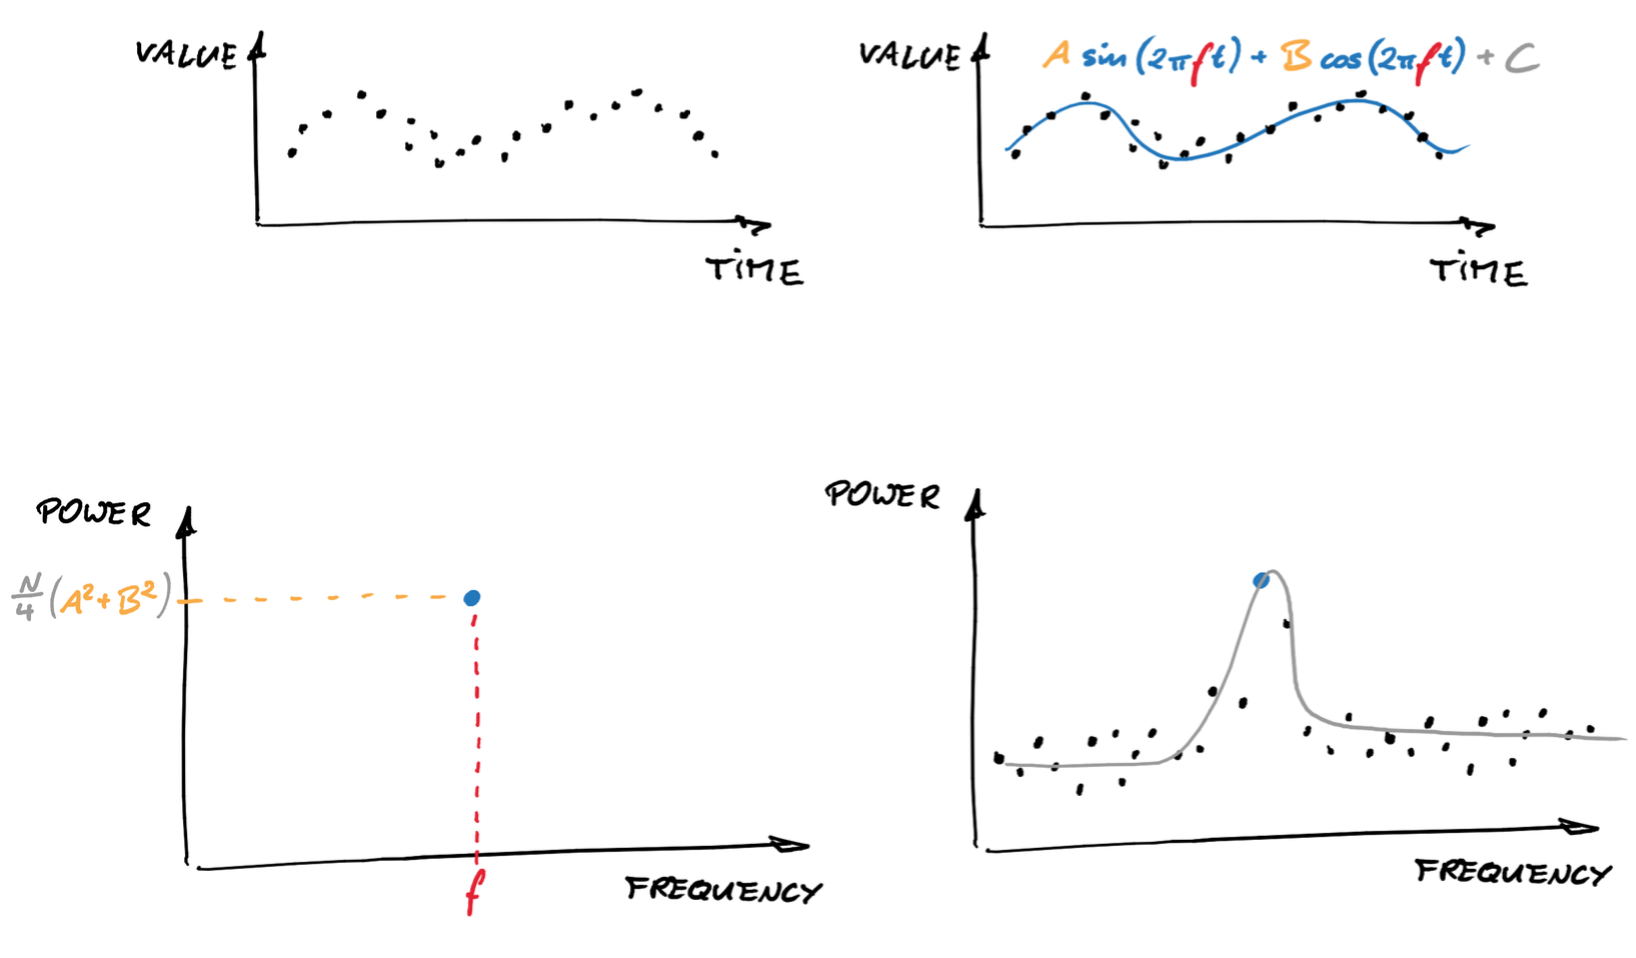
\includegraphics[width=\linewidth]{gfx/axions/LSSA}
  \caption{The construction of an LSSA periodogram.
  The estimate of the LSSA power at the frequency $f$ is the amplitude of the least-squares fit of a harmonic oscillation of that frequency to the time-series (with a normalisation factor).
  The LSSA periodogram, an estimate of the power spectrum, is the LSSA power evaluated for a number of frequencies.}\label{fig:LSSA_overview}
\end{figure}

In order to evaluate the LSSA periodogram at a circular frequency $\omega$, a linear least-squares fit (hence the name) is performed to the data with a function
\marginpar{LSSA, in contrast to the fast Fourier transform (FFT), does not require windowing, because it is explicitly phase-aware.}
\begin{equation}
  A\,\cos(\omega t) + B\,\sin(\omega t) + C \ ,
\end{equation}
where $A$, $B$ and $C$ are free parameters. The estimator of power $P(\omega)$ is then defined as
\begin{equation}
  P(\omega) := \frac{N}{4} \, \left( A^2 + B^2 \right) \ ,
\end{equation}
where $N$ is the number of data points. Different normalisations may be used.
\marginpar{The noise bed is flat part of periodogram due to random noise. If there is a signal, it is said to ``rise out of the noise bed''.}
Here the one of~\cite{Scargle1982} is used, where the height of $\sqrt{P(\omega)}$ at the noise bed corresponds to the size of the error-bars squared, if they are all equal. A graphical overview of the method is shown in Fig.\,\ref{fig:LSSA_overview}. Throughout the analysis the figure of merit is either the power $P(\omega)$ or, interchangeably, its square root---amplitude. The latter has conveniently the same unit as the time series.

\begin{figure}
  \centering 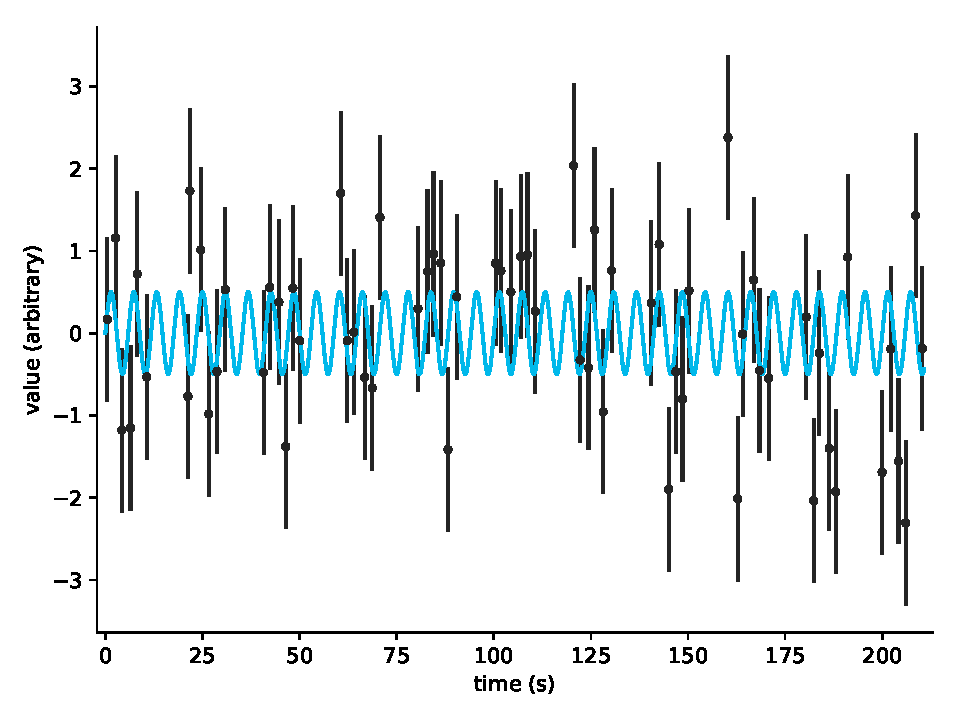
\includegraphics[width=0.8\linewidth]{gfx/axions/basic_signal.pdf}
  \caption{A toy signal generated just for the purpose for explaining the general scheme of the periodogram analysis. A harmonic signal (blue) was used to generate unevenly spaced data points (black). Each point was drawn from a normal distribution centred at the blue curve and a unit width. \note{Remove the legend.}}\label{fig:basic_signal}
\end{figure}

We will now follow an analysis of a toy time series, shown in Fig.\,\ref{fig:basic_signal}. The time series had been fabricated as simulated measurements of an oscillating signal of a frequency \SI{0.17}{\hertz} and an amplitude equal to \num{0.7} in an arbitrary unit.
The series has already some properties of the actual dataset. The measurements are not equally spaced; they are randomly grouped in \SI{10}{\second} long bunches, around \SI{20}{\second} apart. Inside a bunch a ``measurement'' is taken every \SI{2}{\second} with a \SI{0.3}{\second} jitter. The length of each measurement is \SI{1}{\second} with a \SI{0.1}{\second} jitter. The error-bars are all size one in the arbitrary unit. Each ``measurement'' averaged the signal over its duration.

The immediate question arising when evaluating the LSSA periodogram is: for which frequencies to evaluate the power? In a case of evenly-spaced series the upper limit is the Nyquist frequency, equal to the half of the sampling rate~\cite{Shannon1949}.
It is not the case when the sampling is not uniform. In practice, we can expect little sensitivity to oscillations faster than the period over which each signal is averaged, \SI{1}{\second} in the example. On the low side the limit is zero, which corresponds to the constant offset (a least-squares fit of a horizontal line, which is equivalent to calculating the average of the points). The value of the periodogram at zero is usually not plotted.

\begin{figure}
  \centering 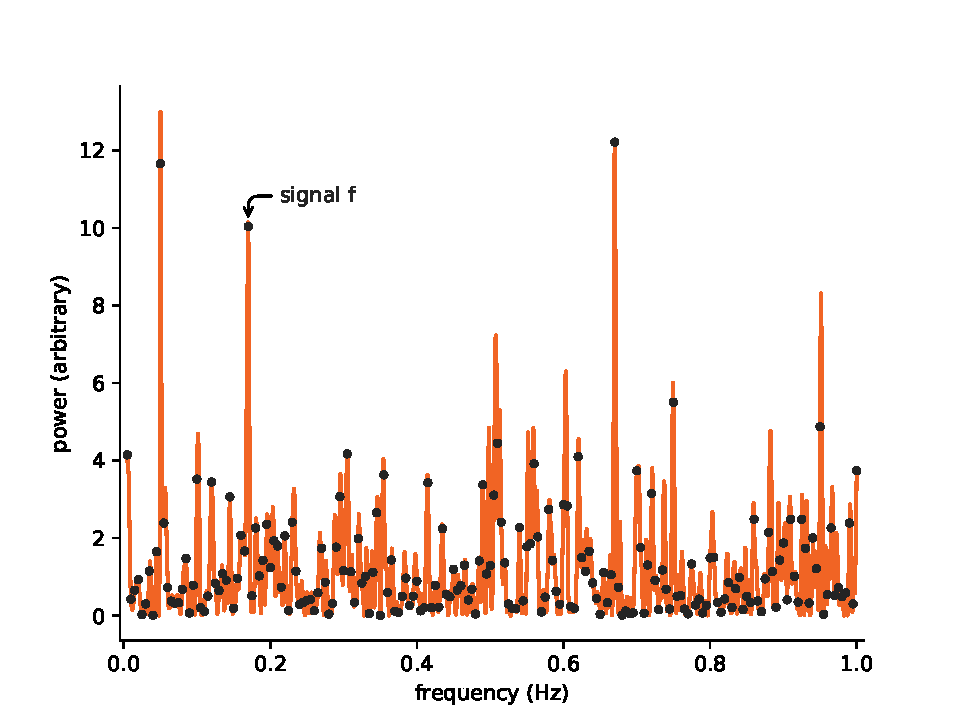
\includegraphics[width=\linewidth]{gfx/axions/basic_periodogram.pdf}
  \caption{Two periodograms of the time series in Fig.\,\ref{fig:basic_signal}. One evaluated at frequencies with a spacing equal to the spectral resolution (black dots), and one evaluated a thousand times more densely (the orange line).}\label{fig:basic_periodogram}
\end{figure}

When choosing the spacing between the frequencies, the \emph{spectral resolution} is considered, defined as the inverse span of the dataset.
\marginpar{A Fourier transform of a rectangular function is a sinc function. Any signal measured for a finite time in the frequency space is necessarily convoluted with the sinc function.}
It roughly defines the minimal frequency difference between two signals that is distinguishable. A perfectly coherent oscillation produces a cardinal-sine-shaped peak of a width equal to the spectral resolution. \note{citation needed}
In Fig.\,\ref{fig:basic_periodogram} there are two periodograms: a ``sparse'' one evaluated at frequencies spaced a full spectral resolution apart (black dots), and one a thousand times more dense (the orange line).
Each peak visible in the dense line is met with at least one sparse evaluation. However, not for each the point is at the peak's full height, which decreases the sensitivity of the method. As a compromise the frequency spacing is sometimes chosen to be a fraction of the spectral resolution, e.g.\ a tenth~\cite{Debosscher2007}. In this work the spacing of a full spectral resolution was used.

\begin{figure}
  \centering 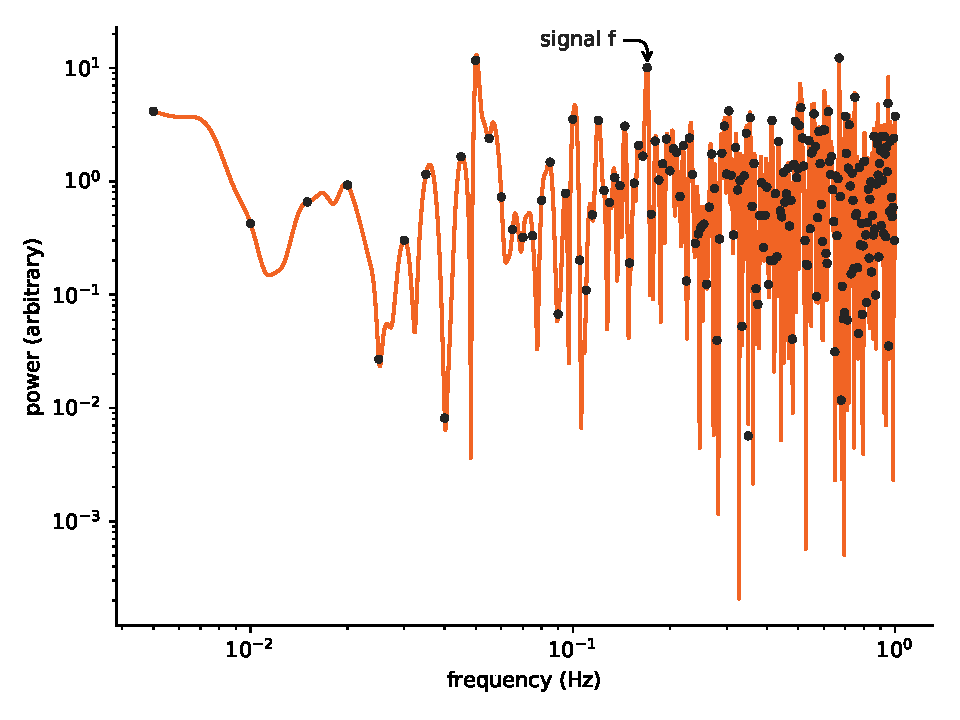
\includegraphics[width=0.8\linewidth]{gfx/axions/basic_periodogram_loglog.pdf}
  \caption{The two periodograms as in Fig.\,\ref{fig:basic_periodogram} plotted on a log-log scale. The range of frequencies where the periodogram is evaluated is extended. The amplitude of the noise appears to be increasing with frequency, but it is not true. Only the density of the evaluated points increases, making the extreme deviations more pronounce.}\label{fig:basic_periodogram_loglog}
\end{figure}

Figure~\ref{fig:basic_periodogram_loglog} shows the same two periodograms in a log-log scale. Additionally, the range of frequencies where the periodogram is evaluated has been extended to show its behaviour in the extremes. The logarithmic scale, albeit useful when the potential signals span orders of magnitude in both frequency and amplitude, can lead to misunderstandings. Specifically, the noise appears to increase in amplitude with frequency, but the effect is purely cognitive. The spacing of the points is linear, so on a logarithmic scale the density of points increases for high amplitude. This makes more of extreme deviations likely to appear per unit area of the plot.%, despite the noise amplitude being the same.

An oscillation in the time series produces a peak in the periodogram. The position of the peak is the frequency of the oscillation, the width corresponds to the coherence of the signal. However, in the periodogram there many peaks besides the one corresponding to the oscillation used when generating the data. Some are even bigger and there are many smaller ones. In the next section we will consider what, besides an oscillating signal, may give rise to a peak. Most importantly, a way of determining whether a peak is caused by an oscillation is presented.




\section{A null hypothesis test}
\label{sec:a_null_hypothesis_test}
Once the periodogram of a time series is calculated, one would like to know whether it contains a statistically significant signature of a signal. For a periodic signal this would be a peak. In our case the really interesting statement is the answer to the question:
\begin{center}
  \emph{How likely is it that the highest peak in the periodogram is not only a random fluctuation?}
\end{center}
This question has already been stated by Scargle~\cite{Scargle1982}. In this section we will be largely following the reasoning he presented, with few important differences.

In order to describe the question mathematically, let us denote the time series under consideration (Fig.\,\ref{fig:basic_signal}) by $D$. The periodogram is then a set of $P^D(\omega_i)$, depicted with a black line in Fig.\,\ref{fig:basic_detection}.
In a uniformly sampled case with equal error bars $P^D(\omega_i)$ is exponentially distributed, for those frequencies where no signal is present~\cite{Scargle1982}. In our, more complicated, case the distribution can be generated by a Monte Carlo (MC) simulation in the following way: a new signal is generated, keeping the time, position and the size of the error bars, but with no underlying signal present---the null hypothesis $H_0$.
The value for each simulated measurement is drawn from a gaussian distribution with the width equal to the size of the error bar. Then the periodogram of the generated time series is calculated. This is repeated a number of times, yielding a set of periodograms, which are used to estimate the probability density function (PDF) of $P(\omega_i)$ for each $i$. The PDF for $\omega = \SI{0.17}{\hertz}$ (the frequency of the signal implanted in the time series) is depicted in the right-hand side of~Fig.\,\ref{fig:basic_detection}.
% In the left-hand side of this figure the 1-, 2- and 3$\upsigma$ bands of the $P(\omega_i)$ PDFs are depicted in shades of green.
In the left-hand side of the figure bands representing the shape of the PDFs for different frequencies (sigma bands, about be explained) are depicted is shades of green.
% the 1-, 2- and 3$\upsigma$ bands of the $P(\omega_i)$ PDFs are depicted in shades of green.
For uniformly sampled data with equal error bars all PDFs would be the same and the bands flat~\cite{Scargle1982}. In our case structures appear, despite absolutely no signal being present in the generated time series.

\begin{figure}
  \centering 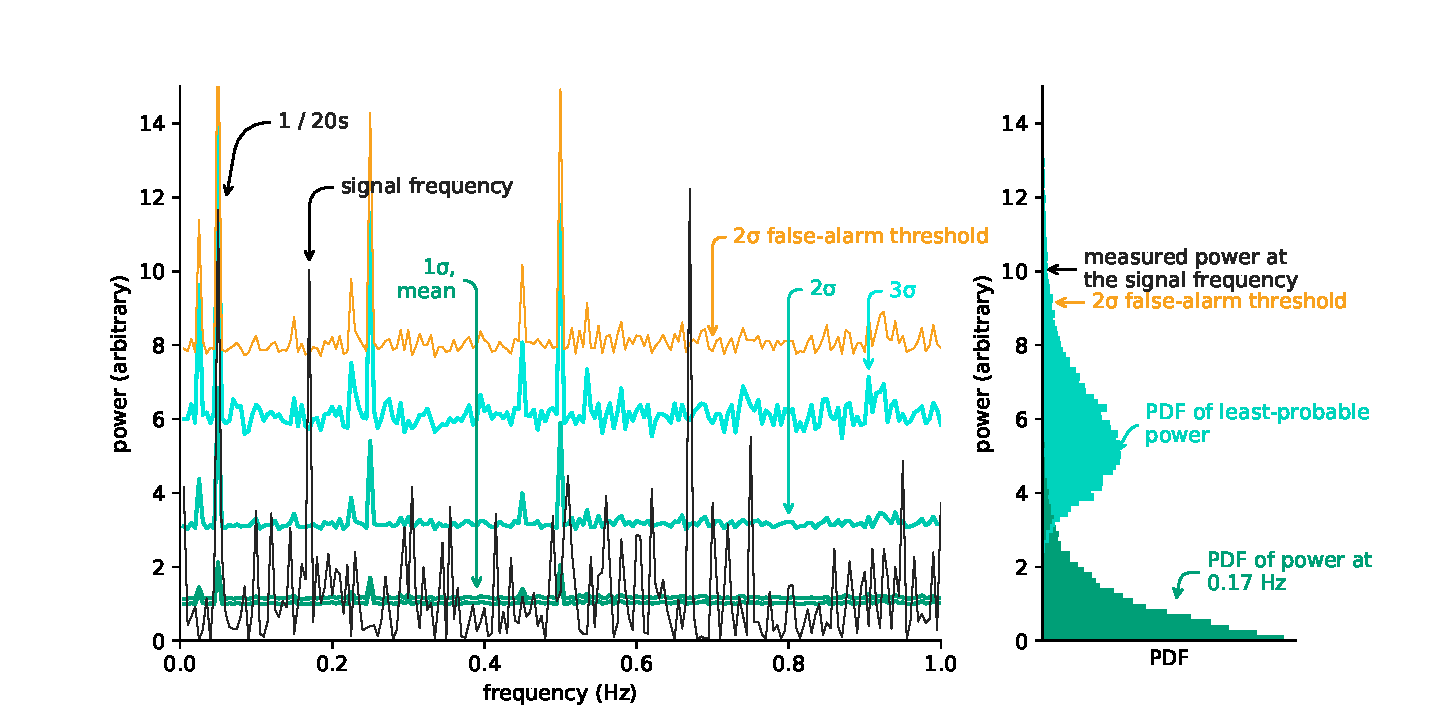
\includegraphics[width=\linewidth]{gfx/axions/basic_detection.pdf}
  \caption{Left-hand side: Juxtaposition of the periodogram of the toy time series (black) and the periodogram PDF under the null hypothesis. For the latter the average and 1-, 2- and 3$\upsigma$ bands are depicted in shades of green. The 2$\upsigma$ global false-alarm threshold is marked in orange. Right-hand side: Aligned with the plot to the left, two PDFs are depicted: the one of the power at \SI{0.17}{\hertz} (the frequency of the signal put into the toy time-series) and the one of the globally least-probable power (across all frequencies).}\label{fig:basic_detection}
\end{figure}

The structures in the $P(\omega_i)$ PDFs are caused solely by the non-uniformity in sampling and in the sizes of the error bars. In particular, we can identify a very large expected rise in power at \SI{0.05}{\hertz}, corresponding exactly to the inverse spacing between the bunches $1 / \SI{20}{\hertz}$, a feature of the toy measurement. A peak is expected in the periodogram to appear at this point, even when there is no significant oscillation of this frequency. This is the reason why the most significant peak should be sought, rather than simply the highest. This conclusion makes the presented reasoning different from the one of Scargle~\cite{Scargle1982}.

%We will be using the Cumulative Density Function (CDF) formalism.
In the formal treatment we denote the cumulative density function (CDF) of the power estimator at the $i$th frequency as $F_i(z)$ ($z$ would be the power estimated at frequency $\omega_i$). In an evenly sampled, signal-free case it has a functional form
\begin{equation}
  \label{eq:local_functional_form}
  F_i(z) = 1 - e^{-z} \ .
\end{equation}
\marginpar{P-value is the probability that at least this much power would arise only as a result of a random fluctuation.}
In our case it can be estimated from the MC simulations. Then the $i$th p-value is directly
\begin{equation} \label{eq:local_p_value}
  p_i = 1 - F_i\left( P^D(\omega_i) \right) \ .
\end{equation}
The most significant peak is the one with the lowest p-value.

\begin{figure}
  \centering
  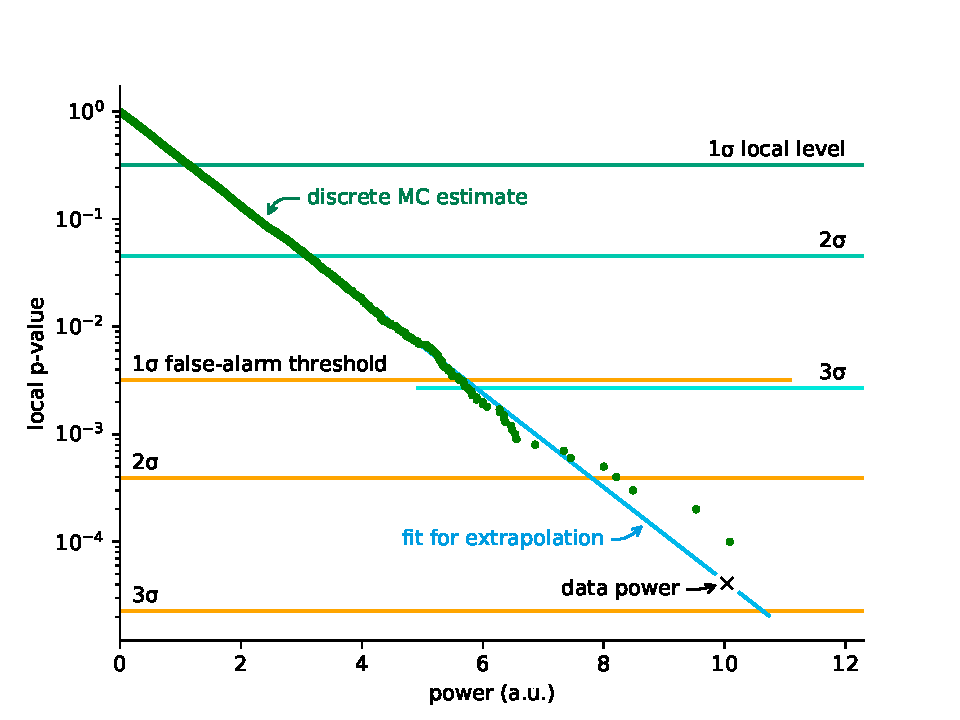
\includegraphics[width=\linewidth]{gfx/axions/MC_estimation_local.pdf}
  \caption{The estimate of the CDF of the power at \SI{0.17}{\hertz}. One-minus-CDF is plotted, so that the use of logarithmic scale details the high-power tail. The discrete estimate from MC samples is depicted with green dots. It is extrapolated with a fit, depicted by the straight blue line. The black cross marks the power in the toy time series at the frequency ($x$ coordinate) and the corresponding local p-value ($y$ coordinate). The local sigma levels are depicted in shades of green and the global ones in orange.}\label{fig:P_best_signal_candidate}
\end{figure}

To construct the discrete CDF estimate all the MC-generated power estimates were sorted into an array. The point of the CDF were obtained by putting the power on the $x$-axis and the place in the sorted array, normalised to one, on the $y$-axis \note{cite}.
\marginpar{The CDF has this advantage over the PDF, that it does not require binning to be estimated.}
The discrete CDF estimate of power, or actually one-minus-CDF, so that the logarithmic $y$-scale can be leveraged to resolve the high-power tail, for the frequency \SI{0.17}{\hertz} is depicted in Fig.\,\ref{fig:P_best_signal_candidate} with the green dots.

When the power in the time series is very high, as it is the case for \SI{0.17}{\hertz} in the example, obtaining the discrete CDF estimate would require many, in some cases unrealistically many, Monte Carlo samples. Generic solutions of this problem are known (see for example section 39.3.2.2 in Ref.\,\cite{PDG2016}). Here, a more specific approach is taken. Motivated by Eq.\,\ref{eq:local_functional_form}, the discrete CDF was extrapolated with a linear fit of the form
\begin{equation}
  F_i(z) = 1 - A_i \, e^{-B_i z} \ ,
\end{equation}
where $A_i$ and $B_i$ are free parameters. The result of the fit is depicted in Fig.\,\ref{fig:P_best_signal_candidate} as a blue line. This line, different for each frequency, was then used to obtain the correspondence between the power and the local p-value for each frequency.


% In order to resolve the tail of the CDF all the way down to 5$\upsigma$ false-alarm threshold, generating at least $10^8$ samples would be`' necessary.  We assume, that even though the CDF will deviate from the strictly derived equations in~\cite{Scargle1982}, the functional form of the tails will be preserved. Under the null hypothesis $F_{P_i}$ has the form $1 - e^{-P}$~\cite{Scargle1982}. For $F^g$ we assume a form of Eq.\,(\ref{eq:Fpmin}), where $N$ is a parameter that we have to fit to account for correlations in the periodogram. Those functional forms can be used to extrapolate tails of CDF estimated with much fewer MC samples.

% First how the local p-values were obtained. In Fig.\,\ref{fig:P_best_signal_candidate} the cumulative distribution function (CDF) \mnote{define CDF somewhere and then just continue to use it. Maybe even a table of abbreviations at the end?} of the power at one frequency (a special one, where the least probable peak is). CDF has this advantage over the PDF, that it does not require binning to be estimated. To estimate the CDF all the MC-generated power estimates are sorted into an array. Then the discrete CDF estimate is plotted by putting the power on the x-axis and the place in the sorted array, normalised to one, on the y-axis. Fig.\,\ref{fig:P_best_signal_candidate} actually shows $1 - \mathrm{CDF}$, so that the logarithmic y-scale can be leveraged to resolve the high-power tail. The plot also includes a extrapolating fit line and false-alarm thresholds, which we now proceed to explain.
P-values are often expressed in terms of $n\upsigma$, relating them to the ones of the normal distribution at integer multiples $n$ of its width $\upsigma$:
\begin{equation}
  \text{p-value} = \mathrm{erfc}\left( \frac{n}{\sqrt{2}} \right)\ ,
\end{equation}
where $\mathrm{erfc}$ is the complementary error function (intuitively understood as ``one minus the integral of the gaussian distribution''). The 1, 2 and 3$\upsigma$ levels of the power distribution are marked in shades of green in Figs.\,\ref{fig:basic_detection} and~\ref{fig:P_best_signal_candidate}.

In the periodogram of the toy signal there are 15 peaks with p-values on a 2$\upsigma$ level. Na\"\i vely, this may seem to be very improbable---a 2$\upsigma$ event is a five-in-a-hundred one. This is the so-called \emph{look-elsewhere effect}~\cite{PDG2016}, best explained as follows: a one-in-a-thousand event in a system is not a surprise, if it occurs in one of a thousand different systems. By looking at the Fig.\,\ref{fig:basic_detection} and comparing the periodogram of the signal with the sigma bands one essentially performs many, as many as the number of frequencies, largely independent statistical tests, cherry-picking among them the most significant peaks. The p-values $p_i$ are called \emph{local}, because they only measure the local significance at $\omega_i$.

There is an another intuitive way of understanding this phenomenon. The height of the most significant peak is a statistic itself. Its distribution can also be estimated from the MC-generated null hypothesis signals. The distribution is depicted on the right-hand size in Fig.\,\ref{fig:basic_detection}. Even when no signal is present, the most significant peak will most of the times have a height placing it between 2- and 3$\upsigma$ local significance bands.

Let us now consider more formally the local p-value of the most significant peak: $p_\text{min} \, | H_0$ and its CDF\@. If the points of the periodogram were perfectly uncorrelated, this would be a simple case of many hypothesis testing~\cite{Algeri2016}. The CDF of the maximum of a set of uncorrelated variables is a product of their CDFs~\cite{Papoulis2002} and the local p-values $p_i$ are, by definition, uniformly distributed. So in this case we have
\begin{align}\label{eq:Fpmin}
  F_p(p) &= p \\
  F_{p_\text{max}}(p) &= p^N \ .
\end{align}
with $p' := 1 - p$:
\begin{equation}
  F_{p_\text{min}}(p) = 1 - F_{p'_\text{max}}(p') = 1 - {(1 - p)}^N \ ,
  \label{eq:global_CDF_functional_form}
\end{equation}
where $N$ is the number of frequencies tested.
% We Correlations in the periodogram, for example due to non-uniform sampling of the time-series, effectively lower $N$. If three dice are rolled in a way that two always give the same result, this is the same as rolling two dice when minimum roll is concerned.
The CDF of $p_\text{min} \, | H_0$, which we call $F^g$, can be estimated from the MC-generated data. Then the \emph{global} p-value is given by
\begin{equation}
  p^g = F^g(p_\text{min}^D) \ ,
\end{equation}
where $p_\text{min}^D$ is the minimal local p-value in the data set.

\begin{figure}
  \centering
  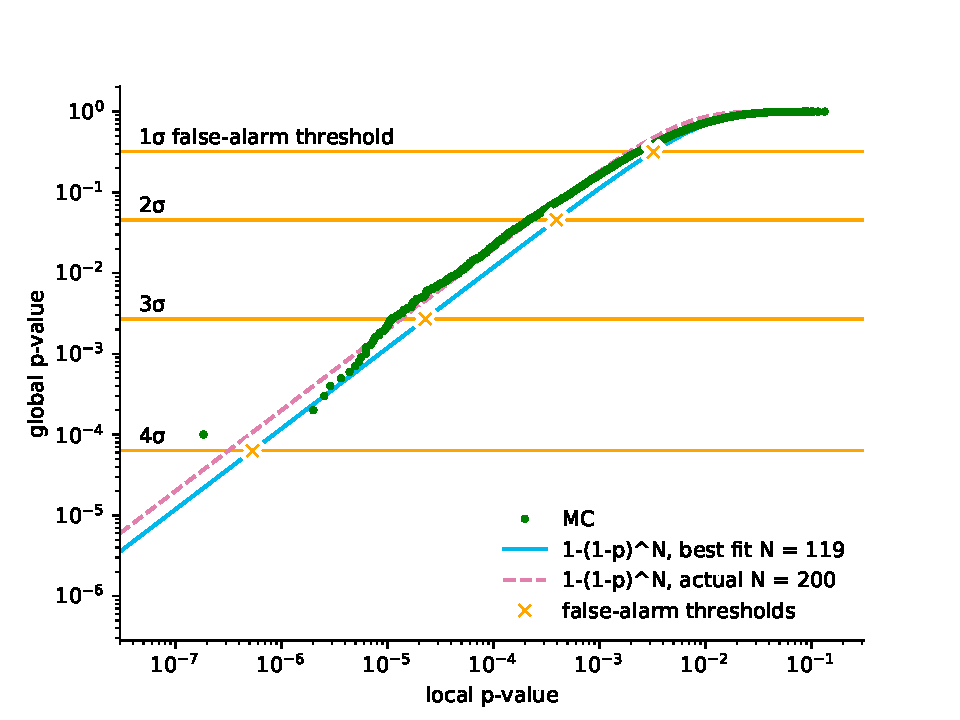
\includegraphics[width=\linewidth]{gfx/axions/MC_estimation_global.pdf}
  \caption{Quantitative illustration of the look-elsewhere effect in the toy data set. The discrete CDF estimate of the lowest local p-value, under the assumption of the null hypothesis, is plotted. For the given lowest local p-value in a periodogram the line gives the corresponding global p-value. The CDF for the case of perfectly uncorrelated power estimates (Eq.\,\ref{eq:global_CDF_functional_form} with $N=200$) is depicted with a pink dashed line. The blue line depicts the best-fit CDF with $N=199$.
  \note{Make nice descriptions to match Fig.\,\ref{fig:P_best_signal_candidate}. And get rid of orange crosses.}}\label{fig:P_look-elsewhere}
\end{figure}

The discrete estimate of $p_\text{min} \, | H_0$ CDF is depicted with green dots in Fig.\,\ref{fig:P_look-elsewhere}. It was obtained by generating many periodograms under the assumption of $H_0$, evaluating the p-value of the most significant peak in each, and then ordering the p-values. The plot has the local p-value on the $x$-axis and the normalised position in the ordered array on the $y$-axis.
As in the case of the local p-value estimation, in order to access the low-probability tail without straining the computational effort the functional form of the CDF was used.
If the power estimates for all the of $N$ tested frequencies are uncorrelated the CDF would be given exactly by Eq.\,\ref{eq:global_CDF_functional_form}.
However, it cannot be guaranteed that the power estimates at different frequencies are independent in a case of a periodogram of an unevenly sampled time series.
Instead, the parameter $N$ was obtained by fitting a curve described by Eq.\,\ref{eq:global_CDF_functional_form} to the discrete CDF estimate. CDFs corresponding to both values of $N$, the actual number of frequencies and the fitted one, are depicted in Fig.\,\ref{fig:P_look-elsewhere}.

% As in the case of the local p-value estimation, to access the low-probability tail without straining the computational effort the CDF has been extrapolated with a fit. Equation~(\ref{eq:global_CDF_functional_form}) was used as the model, $N$ having been the free fit parameter.



% To reduce the computational effort we exploit the fact, that we know the expected functional form of the CDF\@:
% \begin{equation}
%   F(p) = 1 - {(1-p)}^N\ ,
% \end{equation}
% \mnote{Ref.\,for the formula? PDF statistics? Scargle?}
% where $N$ is the total number of frequencies. This corresponds to $N$ \emph{independent} statistical tests. We refrain from using for $N$ the actual number of frequencies, \num{156198}, because we cannot guarantee that the power estimates at different frequencies are independent\footnote{They are in a case of periodograms of evenly sampled series}. Instead, we fit $N$ to the observed CDF obtaining \num{177844}. CDFs corresponding to both values of $N$ are depicted in Fig.\,\ref{fig:P_look-elsewhere} and are almost overlapping.

Going further, the global false-alarm thresholds can be determined. The \emph{global} threshold p-value we call $p^{\,g}_\text{f.a.}$. The corresponding threshold for the local p-value is
\begin{equation}
  p_\text{f.a.} = {\left( F^{\,g} \right)}^{-1}(p^{\,g}_\text{f.a.}) \ .
\end{equation}
For each frequency the threshold local p-value gives the threshold power:
\begin{equation}
  P^\text{\,f.a.}_i = F_{P_i}^{-1}(1 - p_\text{f.a.}) \ .
\end{equation}
The p-values for integer sigma levels are depicted in if Fig.\,\ref{fig:P_look-elsewhere} in orange.
\marginpar{Note, that the local sigma levels in Fig.\,\ref{fig:P_best_signal_candidate} and global ones in Fig.\,\ref{fig:P_look-elsewhere} have the same position on the $y$ axis.}
The 2$\upsigma$ false-alarm threshold for the toy time-series is depicted in Fig.\,\ref{fig:basic_detection}, also in orange. It conveys an intuitive massage: a single crossing of the 2$\upsigma$ false-alarm threshold anywhere would mean a 2$\upsigma$ confidence, that there is a statistically significant signal in the time-series (which there is). To claim a discovery of a significant oscillating signal, the false-alarm probability has to be at most in the range of \num{2.87e-7} (5$\upsigma$)~\cite{PDG2016}.

In summary, the difficulty lies in determining the false-alarm thresholds. Then the detection boils down to comparing the periodogram of the time series to the thresholds on a plot similar to the one in Fig.\,\ref{fig:basic_detection}.

% Once every MC-generated power estimate has a local p-value associated with it, we find for each generated periodogram the minimal local p-value and treat it as a statistic in itself. We estimate the CDF of the minimal local p-value. The result is plotted in Fig.\,\ref{fig:P_look-elsewhere}. The plot can be understood in the following way: it states how probable it is (y-axis) for a peak of a given local significance (x-axis) to occur anywhere in a periodogram. In other words, the y-axis corresponds to the \emph{global} p-value. The global p-value for an $n\,\sigma$ level is given by:
% \begin{equation}
%   \mathrm{erfc}\left( \frac{n}{\sqrt{2}} \right)\ ,
% \end{equation}
% where $\mathrm{erfc}$ is the complementary error function (intuitively understood as ``one minus the integral of the gaussion distribution''). We mark the global p-values corresponding to $1,\ldots,5\sigma$ levels and via the CDF find the corresponding local p-value thresholds.

% In order to resolve the tail of the CDF all the way down to 5$\upsigma$ false-alarm threshold, generating at least $10^8$ samples would be`' necessary. Generic solutions of this problem are known (see for example section 39.3.2.2 \emph{The look-elsewhere effect} in~\cite{PDG2016}). Here, a more specific approach is taken. We assume, that even though the CDF will deviate from the strictly derived equations in~\cite{Scargle1982}, the functional form of the tails will be preserved. Under the null hypothesis $F_{P_i}$ has the form $1 - e^{-P}$~\cite{Scargle1982}. For $F^g$ we assume a form of Eq.\,(\ref{eq:Fpmin}), where $N$ is a parameter that we have to fit to account for correlations in the periodogram. Those functional forms can be used to extrapolate tails of CDF estimated with much fewer MC samples.

% We see, that the discrete estimate from the MC simulation can only go down to the $2\sigma$ false-alarm threshold. To go lower would require many more MC samples. To observe a single $5\sigma$ event, roughly one-in-a-million, needs typically a million samples. To reduce the computational effort we exploit the fact, that we know the expected functional form of the CDF\@:
% \begin{equation}
%   F(p) = 1 - {(1-p)}^N\ ,
% \end{equation}
% \mnote{Ref.\,for the formula? PDF statistics? Scargle?}
% where $N$ is the total number of frequencies. This corresponds to $N$ \emph{independent} statistical tests. We refrain from using for $N$ the actual number of frequencies, \num{156198}, because we cannot guarantee that the power estimates at different frequencies are independent\footnote{They are in a case of periodograms of evenly sampled series}. Instead, we fit $N$ to the observed CDF obtaining \num{177844}. CDFs corresponding to both values of $N$ are depicted in Fig.\,\ref{fig:P_look-elsewhere} and are almost overlapping.

% Now for each frequency the local p-values corresponding the false-alarm thresholds are known. They are depicted in Fig.\,\ref{fig:P_best_signal_candidate}. There, the power CDF (at this frequency) can be used to express the thresholds in power or evaluate the global significance of an arbitrary power. Here, too, the problem is that the discretely estimated CDF does not reach far enough in the tails, and, again, we exploit the functional form to extrapolate the CDF. We expect the power to be exponentially distributed in a no-signal case \cite{Scargle1982}, which corresponds to a straight line on the CDF plot with a logarithmic y-scale.


% In Fig.\,\ref{fig:ILL_detection} we present the periodogram of a fake ILL dataset (generated with the same run timings and uncertainties as in the real dataset, with run EDM values generated according to gaussian distribution with mean of $0$ and standard deviation equal to that run's uncertainty). We decided not to analyse the real data set until we are fully happy with the method.
%
% \begin{figure}[h!]
%   \begin{center}
%     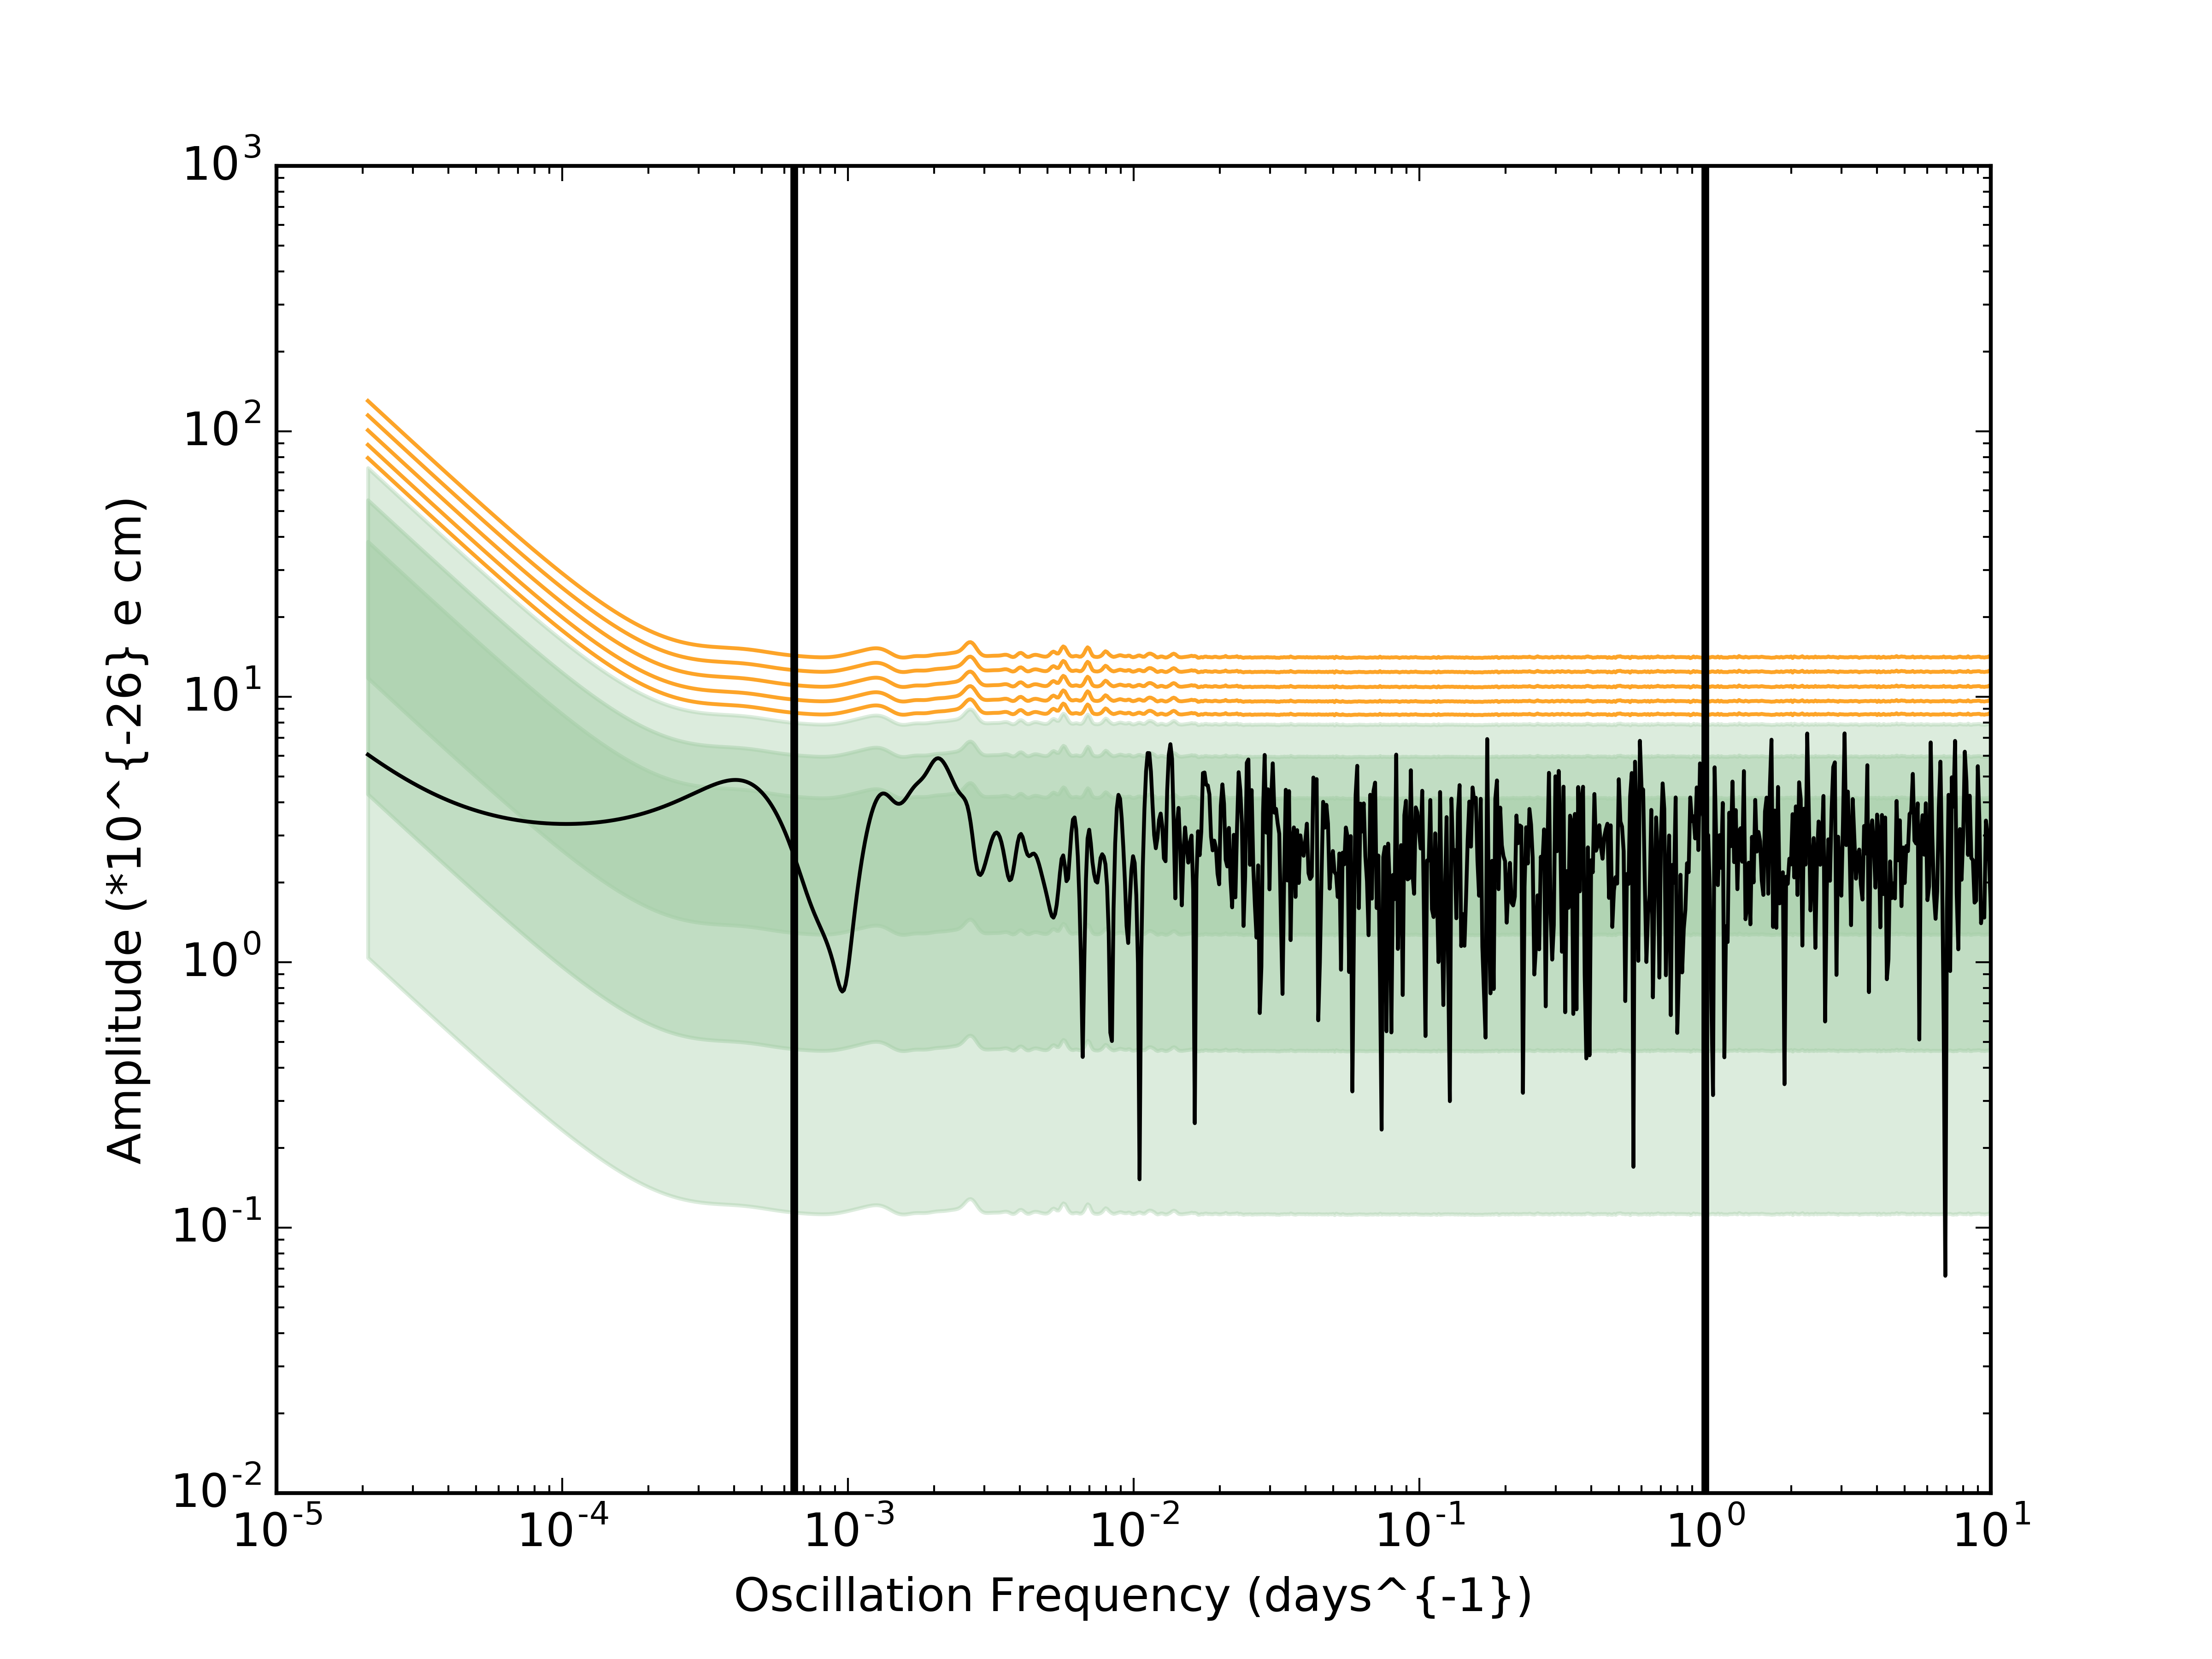
\includegraphics[width=\columnwidth]{gfx/axions/ILL_detection_Periodogram.png}
%     \caption{Periodogram of a fake ILL dataset. The green bands represent the distribution of the periodogram given the null hypothesis. The orange lines are 1-, 2-, 3-, 4-, 5--sigma false--alarm thresholds.}
%     \label{fig:ILL_detection}
%   \end{center}
% \end{figure}



% \section{False-alarm thresholds}
% \mnote{In this section we will dive in more deeply into statistics associated with the data.}

% Remind: for each of the three data sets we have a periodogram, one value for the power estimate for each frequency. Then we have a collection of simulated periodograms, many power estimates for each frequency, generate1d assuming the null hypothesis --- only white noise in the data.

% First how the local p-values were obtained. In Fig.\,\ref{fig:P_best_signal_candidate} the cumulative distribution function (CDF) \mnote{define CDF somewhere and then just continue to use it. Maybe even a table of abbreviations at the end?} of the power at one frequency (a special one, where the least probable peak is). CDF has this advantage over the PDF, that it does not require binning to be estimated. To estimate the CDF all the MC-generated power estimates are sorted into an array. Then the discrete CDF estimate is plotted by putting the power on the x-axis and the place in the sorted array, normalised to one, on the y-axis. Fig.\,\ref{fig:P_best_signal_candidate} actually shows $1 - \mathrm{CDF}$, so that the logarithmic y-scale can be leveraged to resolve the high-power tail. The plot also includes a extrapolating fit line and false-alarm thresholds, which we now proceed to explain.

% \begin{figure}
%   \centering
%   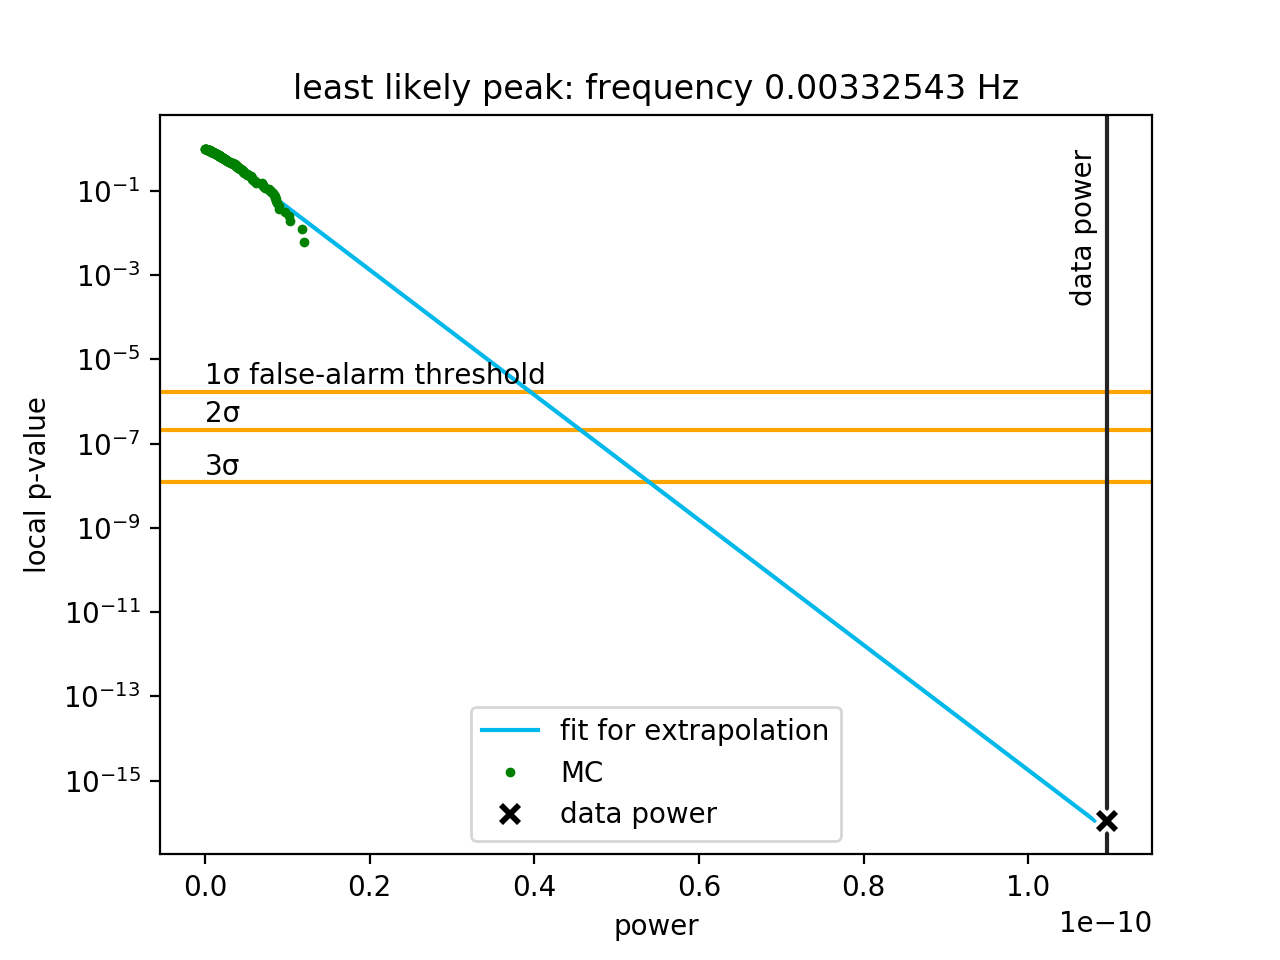
\includegraphics[width=0.9\linewidth]{gfx/axions/P_best_signal_candidate.png}
%   \caption{1 - CDF for the parallel data set. This provides the power to local p-value transition, for each frequency separately. The extrapolation based on Eq.\ldots is shown.}
%   \label{fig:P_best_signal_candidate}
% \end{figure}

% Once every MC-generated power estimate has a local p-value associated with it, we find for each generated periodogram the minimal local p-value and treat it as a statistic in itself. We estimate the CDF of the minimal local p-value. The result is plotted in Fig.\,\ref{fig:P_look-elsewhere}. The plot can be understood in the following way: it states how probable it is (y-axis) for a peak of a given local significance (x-axis) to occur anywhere in a periodogram. In other words, the y-axis corresponds to the \emph{global} p-value. The global p-value for an $n\,\sigma$ level is given by:
% \begin{equation}
%   \mathrm{erfc}\left( \frac{n}{\sqrt{2}} \right)\ ,
% \end{equation}
% where $\mathrm{erfc}$ is the complementary error function (intuitively understood as ``one minus the integral of the gaussion distribution''). We mark the global p-values corresponding to $1,\ldots,5\sigma$ levels and via the CDF find the corresponding local p-value thresholds.

% \begin{figure}
%   \centering
%   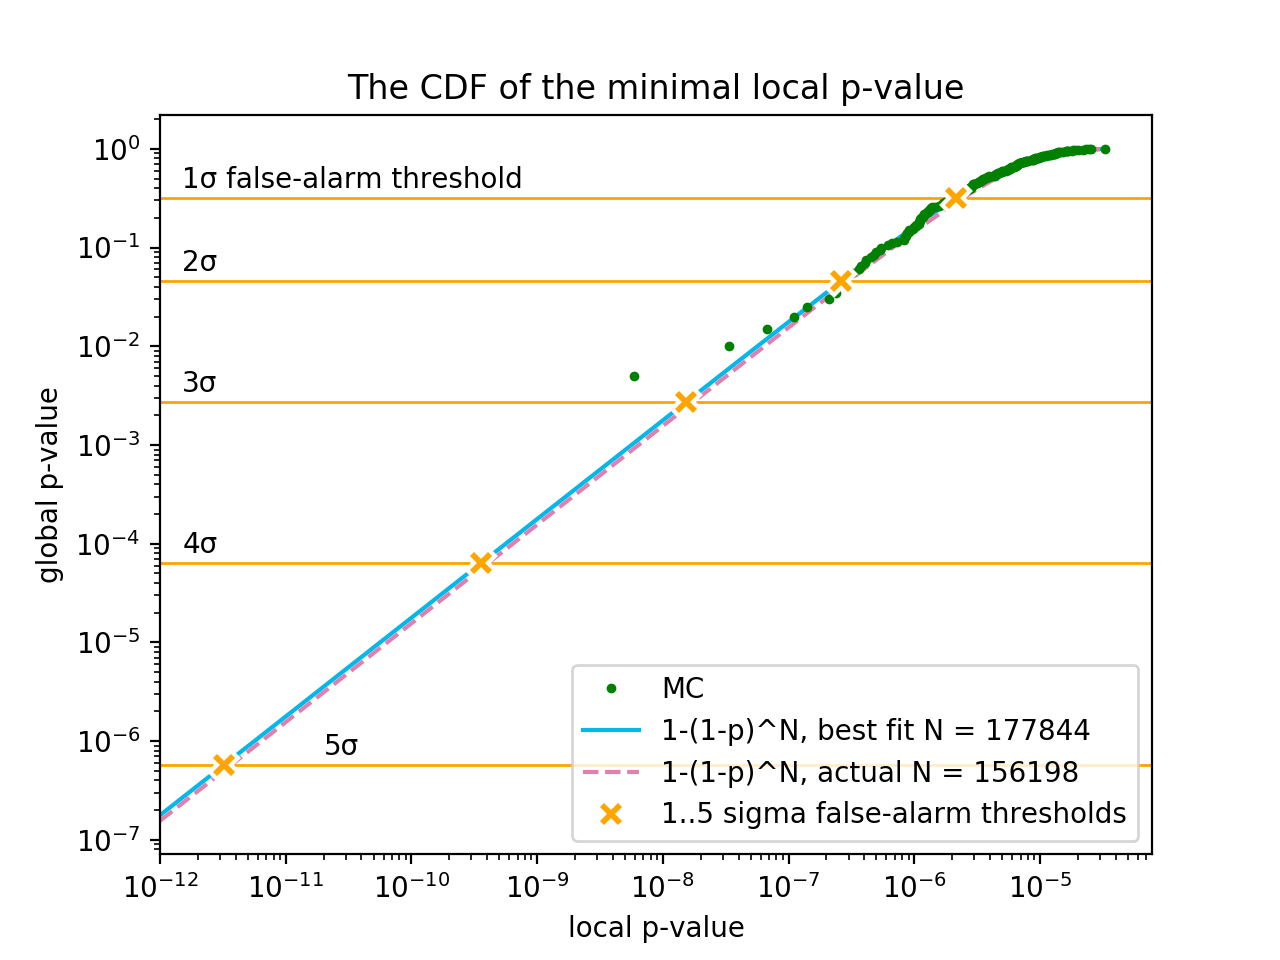
\includegraphics[width=0.9\linewidth]{gfx/axions/P_look-elsewhere.png}
%   \caption{Accounting for the look-elsewhere effect for the parallel dataset. It provides the minimal local p-value---global p-value transition. The fit with the model \dots gives the number of frequencies.}
%   \label{fig:P_look-elsewhere}
% \end{figure}

% We see, that the discrete estimate from the MC simulation can only go down to the $2\sigma$ false-alarm threshold. To go lower would require many more MC samples. To observe a single $5\sigma$ event, roughly one-in-a-million, needs typically a million samples. To reduce the computational effort we exploit the fact, that we know the expected functional form of the CDF\@:
% \begin{equation}
%   F(p) = 1 - (1-p)^N\ ,
% \end{equation}
% \mnote{Ref.\,for the formula? PDF statistics? Scargle?}
% where $N$ is the total number of frequencies. This corresponds to $N$ \emph{independent} statistical tests. We refrain from using for $N$ the actual number of frequencies, \num{156198}, because we cannot guarantee that the power estimates at different frequencies are independent\footnote{They are in a case of periodograms of evenly sampled series}. Instead, we fit $N$ to the observed CDF obtaining \num{177844}. CDFs corresponding to both values of $N$ are depicted in Fig.\,\ref{fig:P_look-elsewhere} and are almost overlapping.

% Now for each frequency the local p-values corresponding the false-alarm thresholds are known. They are depicted in Fig.\,\ref{fig:P_best_signal_candidate}. There, the power CDF (at this frequency) can be used to express the thresholds in power or evaluate the global significance of an arbitrary power. Here, too, the problem is that the discretely estimated CDF does not reach far enough in the tails, and, again, we exploit the functional form to extrapolate the CDF. We expect the power to be exponentially distributed in a no-signal case \cite{Scargle1982}, which corresponds to a straight line on the CDF plot with a logarithmic y-scale.

% The thresholds powers are different for each frequency and are depicted in orange in Fig.\,\ref{fig:axions_PSI_detection}. They provide an intuitive interpretation of the plot: the most significant signal candidate is the one piercing furthest into the false-alarm thresholds. Its statistical significance is equal to the last threshold it crossed.





\section{Signal hypotheses tests}
\label{sec:signal_hypotheses_tests}
Should no claim for a discovery be possible, the next question to ask is:
\begin{center}
  \emph{Which oscillations would produce a visible peak, but did not, and can be thus excluded?}
\end{center}
In order to answer this question the data need to be tested against being compatible with a number of model signal hypotheses. As an oscillation is characterised by its amplitude and frequency, the space of the hypotheses to test is two-dimensional.

\begin{figure}
  \centering 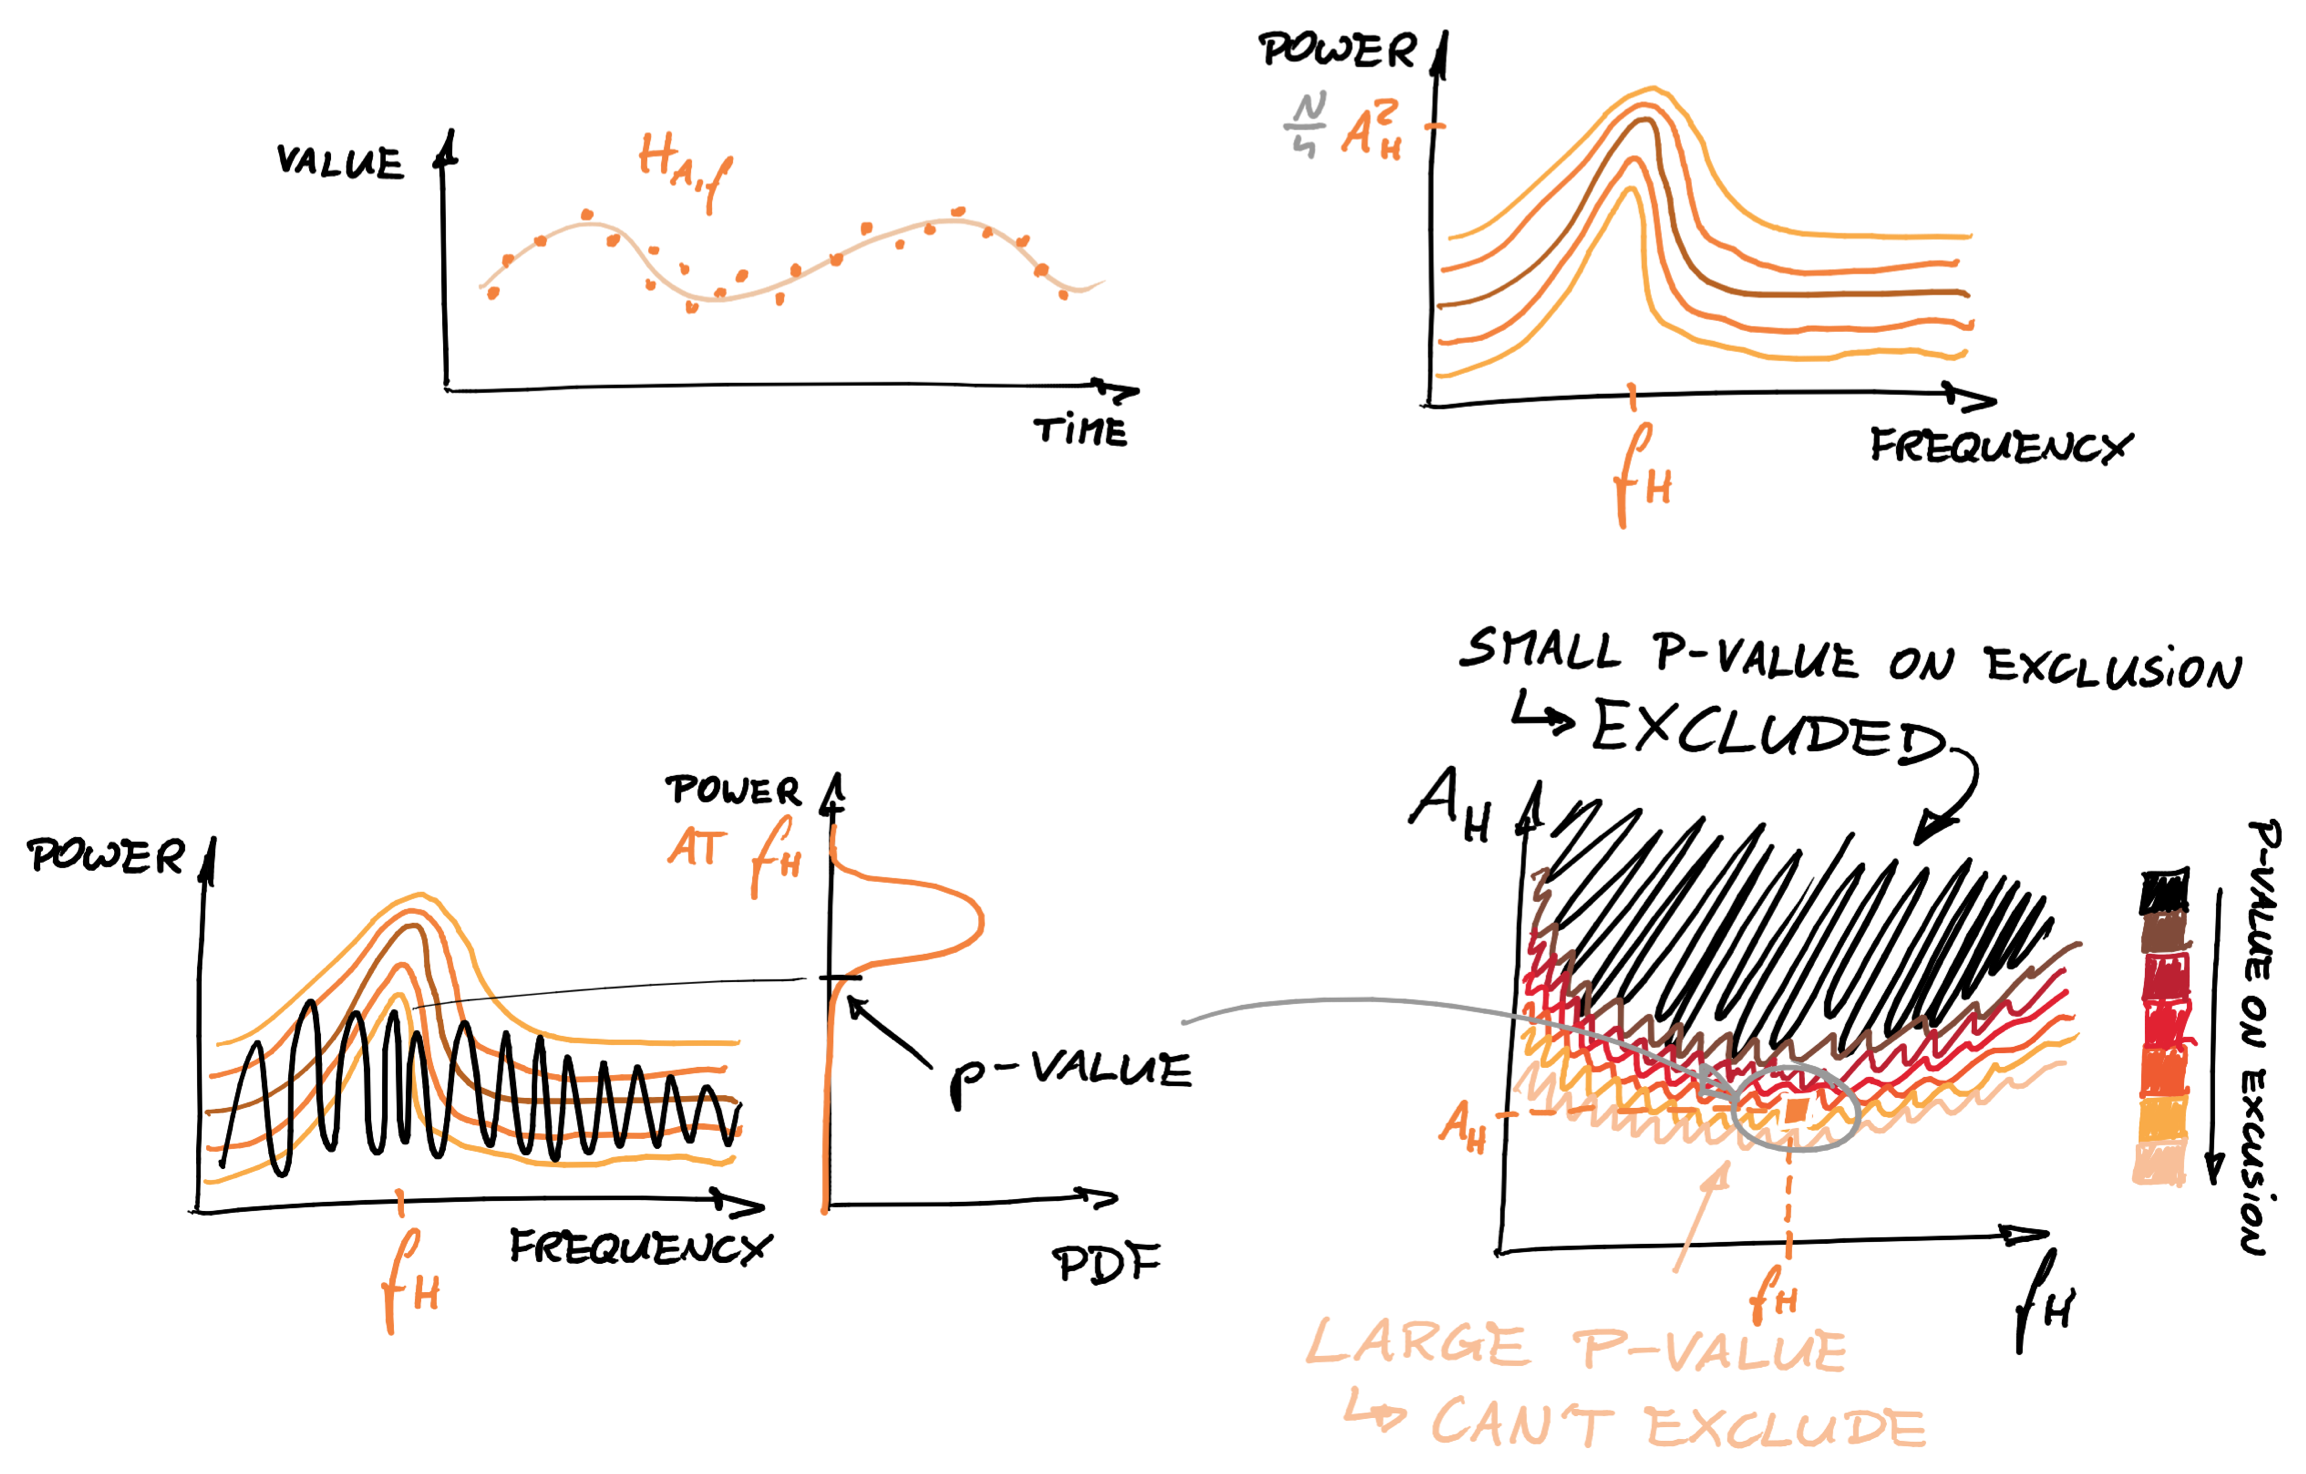
\includegraphics[width=\linewidth]{gfx/axions/exclusion_region.png}
  \caption{The general scheme for the determination of the exclusion region. First, a hypothesis about a signal, parametrised by its amplitude and frequency $f_H$, is assumed. Then, the distribution of the LSSA power at the frequency $f_H$ is estimated under this assumption. The p-value of the time series' power, evaluated against the estimated distribution, is the measure of the confidence level on which the signal hypothesis can be rejected. This is repeated to cover the space of possible signals.}\label{fig:exclusion_region}
\end{figure}

The probability that a hypothetical oscillation of amplitude $A$ and frequency $\omega$ would produce less power at frequency $\omega$ then observed is
\begin{equation}
  % \mathrm{Pr}\left( P(\omega) < P^D(\omega)\ |\, H(\omega, A) \right) \ .
  \Pr\left( P^{H(\omega, A)}(\omega) < P^D(\omega)\ \right) \ .
\end{equation}
This probability is the p-value for the hypothesis $H(\omega, A)$ rejection. The distribution of $P^{H(\omega, A)}(\omega)$ was obtained with the Monte Carlo method in the following way.
A signal was generated with a frequency $\omega$ and amplitude $A$. Then, the LSSA power at the frequency $\omega$, $P^{H(\omega, A)}(\omega)$, was evaluated and compared with the one of the time series $P^D(\omega)$.
This test was repeated for different $\omega$ and $A$, each time covering a pixel of the space of possible hypotheses. The procedure is schematically shown in Fig.\,\ref{fig:exclusion_region}.
The set of hypotheses excluded at most at certain p-value forms an exclusion region. We took the threshold p-value to be \SI{5}{\percent}, which corresponds to the confidence level of \SI{95}{\percent}.

The frequency spectrum is covered much less densely than by the null hypothesis test. This procedure estimates the sensitivity of the measurement, solely determined by the timing and precision of the measurement points. No highly resonant structures are expected to appear therein.
Also, a broader frequency range was covered, logarithmically spaced \SIrange[range-phrase=--]{e-3}{10}{\hertz}, in comparison to linearly spaced \SIrange[range-phrase=--]{5e-3}{1}{\hertz} in the test of the null hypothesis. Thereby the behaviour of sensitivity of the method for extreme frequencies is illustrated.

\marginpar{During the Monte Carlo simulations a perfectly coherent signal is assumed. The width of a real axion-induced peak is not resolvable by the nEDM experiment.}

% \begin{figure}
%   \myfloatalign
%   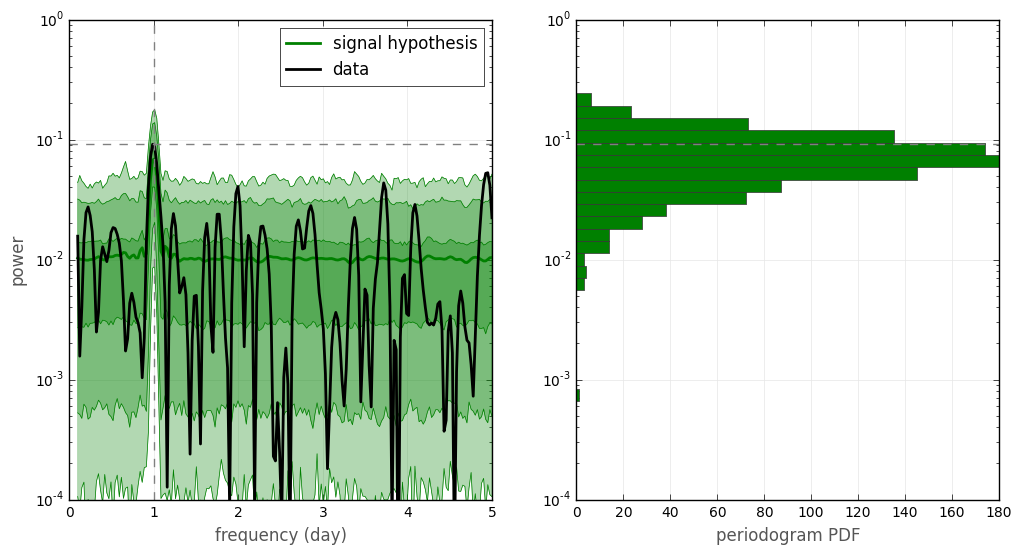
\includegraphics[width=.8\linewidth]{gfx/axions/axionMC_signal_hypothesis_rejection}
%   \caption
%   [...]
%   {
% \textsc{Left:} A periodogram of not--yet--real data on top of distribution of a periodogram of a hypothetical signal (green). \textsc{Right:} The distribution of power of the hypothetical signal at its model frequency.}
%   \label{fig:axions_signal_rejection}
% \end{figure}

\begin{figure}
  \centering
  \subfloat[The test without the use of the CLs method.]
  % The white line connects points of 95\% C.L., surrounding an exclusion region. Note how deep into low amplitudes the line goes for couple of frequencies. See the text for the explanation. \note{Put a white line for the 95\% C.L. exclusion.}]
  {\label{fig:axions_exclusion_noCLs}
  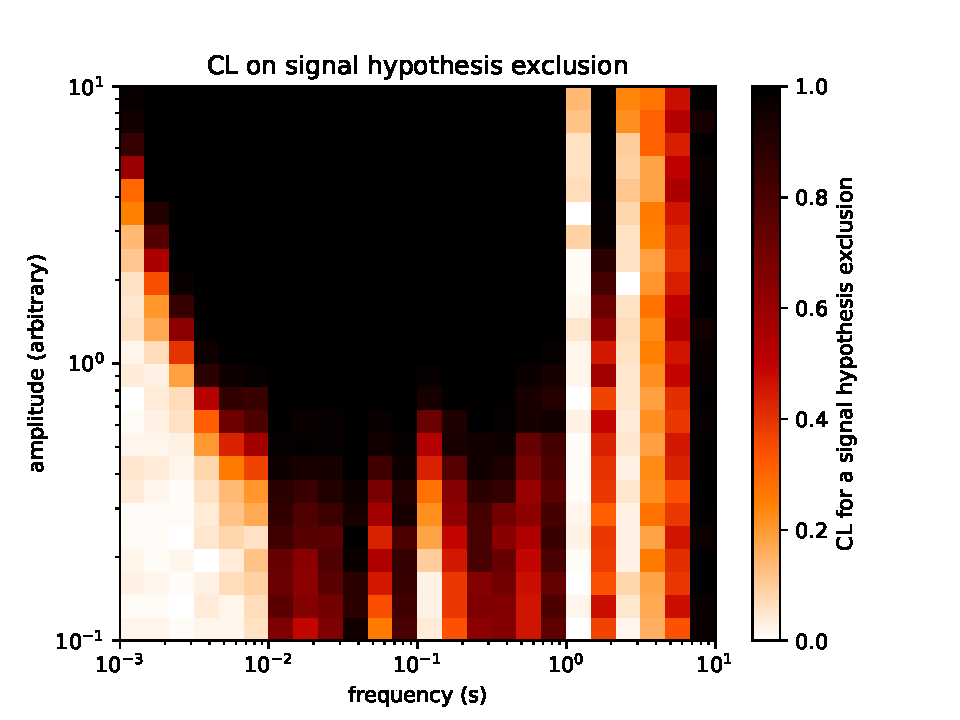
\includegraphics[width=.5\linewidth]{gfx/axions/basic_exclusion_noCls.pdf}}
  \subfloat[The test with the use of the CLs method. Those hypotheses to which the measurement is not sensitive to get a statistical penalty.]
  {\label{fig:axions_exclusion_CLs}
  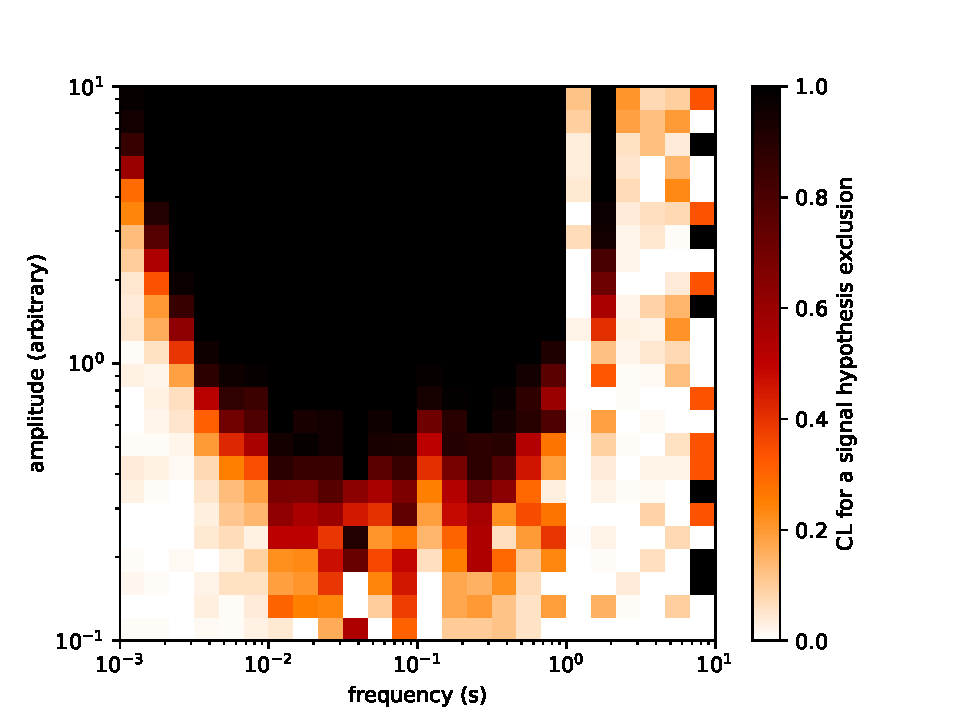
\includegraphics[width=.5\linewidth]{gfx/axions/basic_exclusion.pdf}}
  \caption{The toy time series tested against hypothetical signals. The signal space is spanned by their frequency and amplitude. The colour depicts the confidence level with which the signal can be rejected. The black region is excluded with a high confidence. \note{Put them closer side-by-side, one error bar, remove unnecessary y-ticks. Remove the title on the plot on the left.}}\label{fig:axions_exclusions}
\end{figure}

The result of this procedure applied to the toy time series is presented on the left-hand side in Fig.\,\ref{fig:axions_exclusions}. In the space of possible signals the colour depicts the confidence level for rejecting the signals. The black region, corresponding to high confidence, is excluded. The exclusion region goes down to small amplitudes only in the region between \SI{e-2}{\hertz} (the time series is around \SI{200}{\second} long) and \SI{1}{\hertz} (each of the toy measurements integrated the signal for one second).

\begin{figure}
  \centering 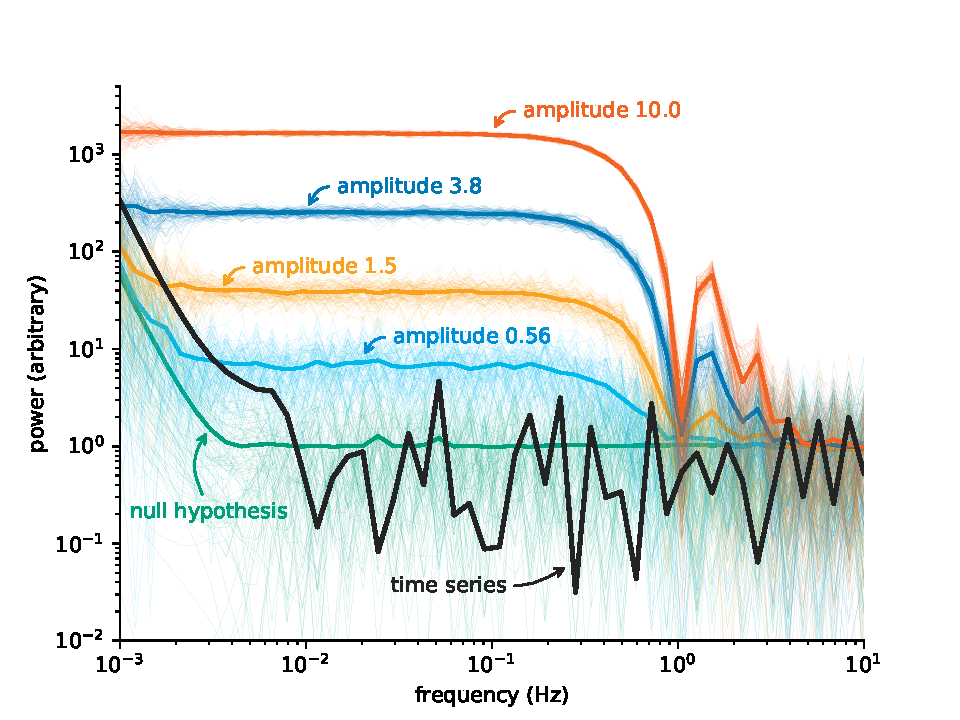
\includegraphics[width=\linewidth]{gfx/axions/basic_exclusion_sensitivity.pdf}
  \caption{For each frequency, the LSSA power of a simulated signal of that frequency is plotted. Different colours correspond to different amplitudes of the signal, in particular no signal, the null hypothesis, is depicted in green. The lines have the interpretation of the height of a peak for different frequencies (the $x$ axis) and amplitudes (colours). The thin lines represent the different simulation outcomes, the thick ones---their average. The black line is the periodogram of the toy time series itself.}\label{fig:sensitivity}
\end{figure}

Figure~\ref{fig:sensitivity} illustrates the mechanism behind the loss of sensitivity for high and low frequencies. The average power obtained for various hypotheses is plotted together with the periodogram of the toy time series. Each coloured line depicts how high a peak caused by a generated signal is, as the function of the frequency of the signal.
% For hypotheses with the same assumed amplitude of oscillation, the amplitude in the periodogram is constant for periods between the separation of the data points and the total length of the data set.
The signal peaks rise distinctly over the null hypothesis' periodogram only in a limited frequency range. Periods significantly longer than the length of the time series (below \SI{e-2}{\hertz}) are difficult to exclude, as it is always possible that the time series is located in an antinode of an extremely slow oscillation. This manifests itself as a high amplitude seen even when the null hypothesis is assumed. On the other end the power for frequencies above \SI{1}{\hertz} is suppressed, because the measurements are not point-like, but rather the oscillation is averaged over a period of \SI{1}{\second}. Only little power is observed, even for very large amplitudes of the signal.

% In particular, it is interesting to consider the difference between the 0 (offset) and the next frequency. Oscillations with a period longer than the span of the time series  appear in the series as a linear drift, if the measurements were taken in the linear part of the sine, or a quadratic change, if taken in the apex. Fitting such an oscillation is then equivalent to looking for a up--to--second--order drift in the data. Naturally, we expect the sensitivity to quickly worsen for these very long oscillations.

\begin{figure}
  \centering 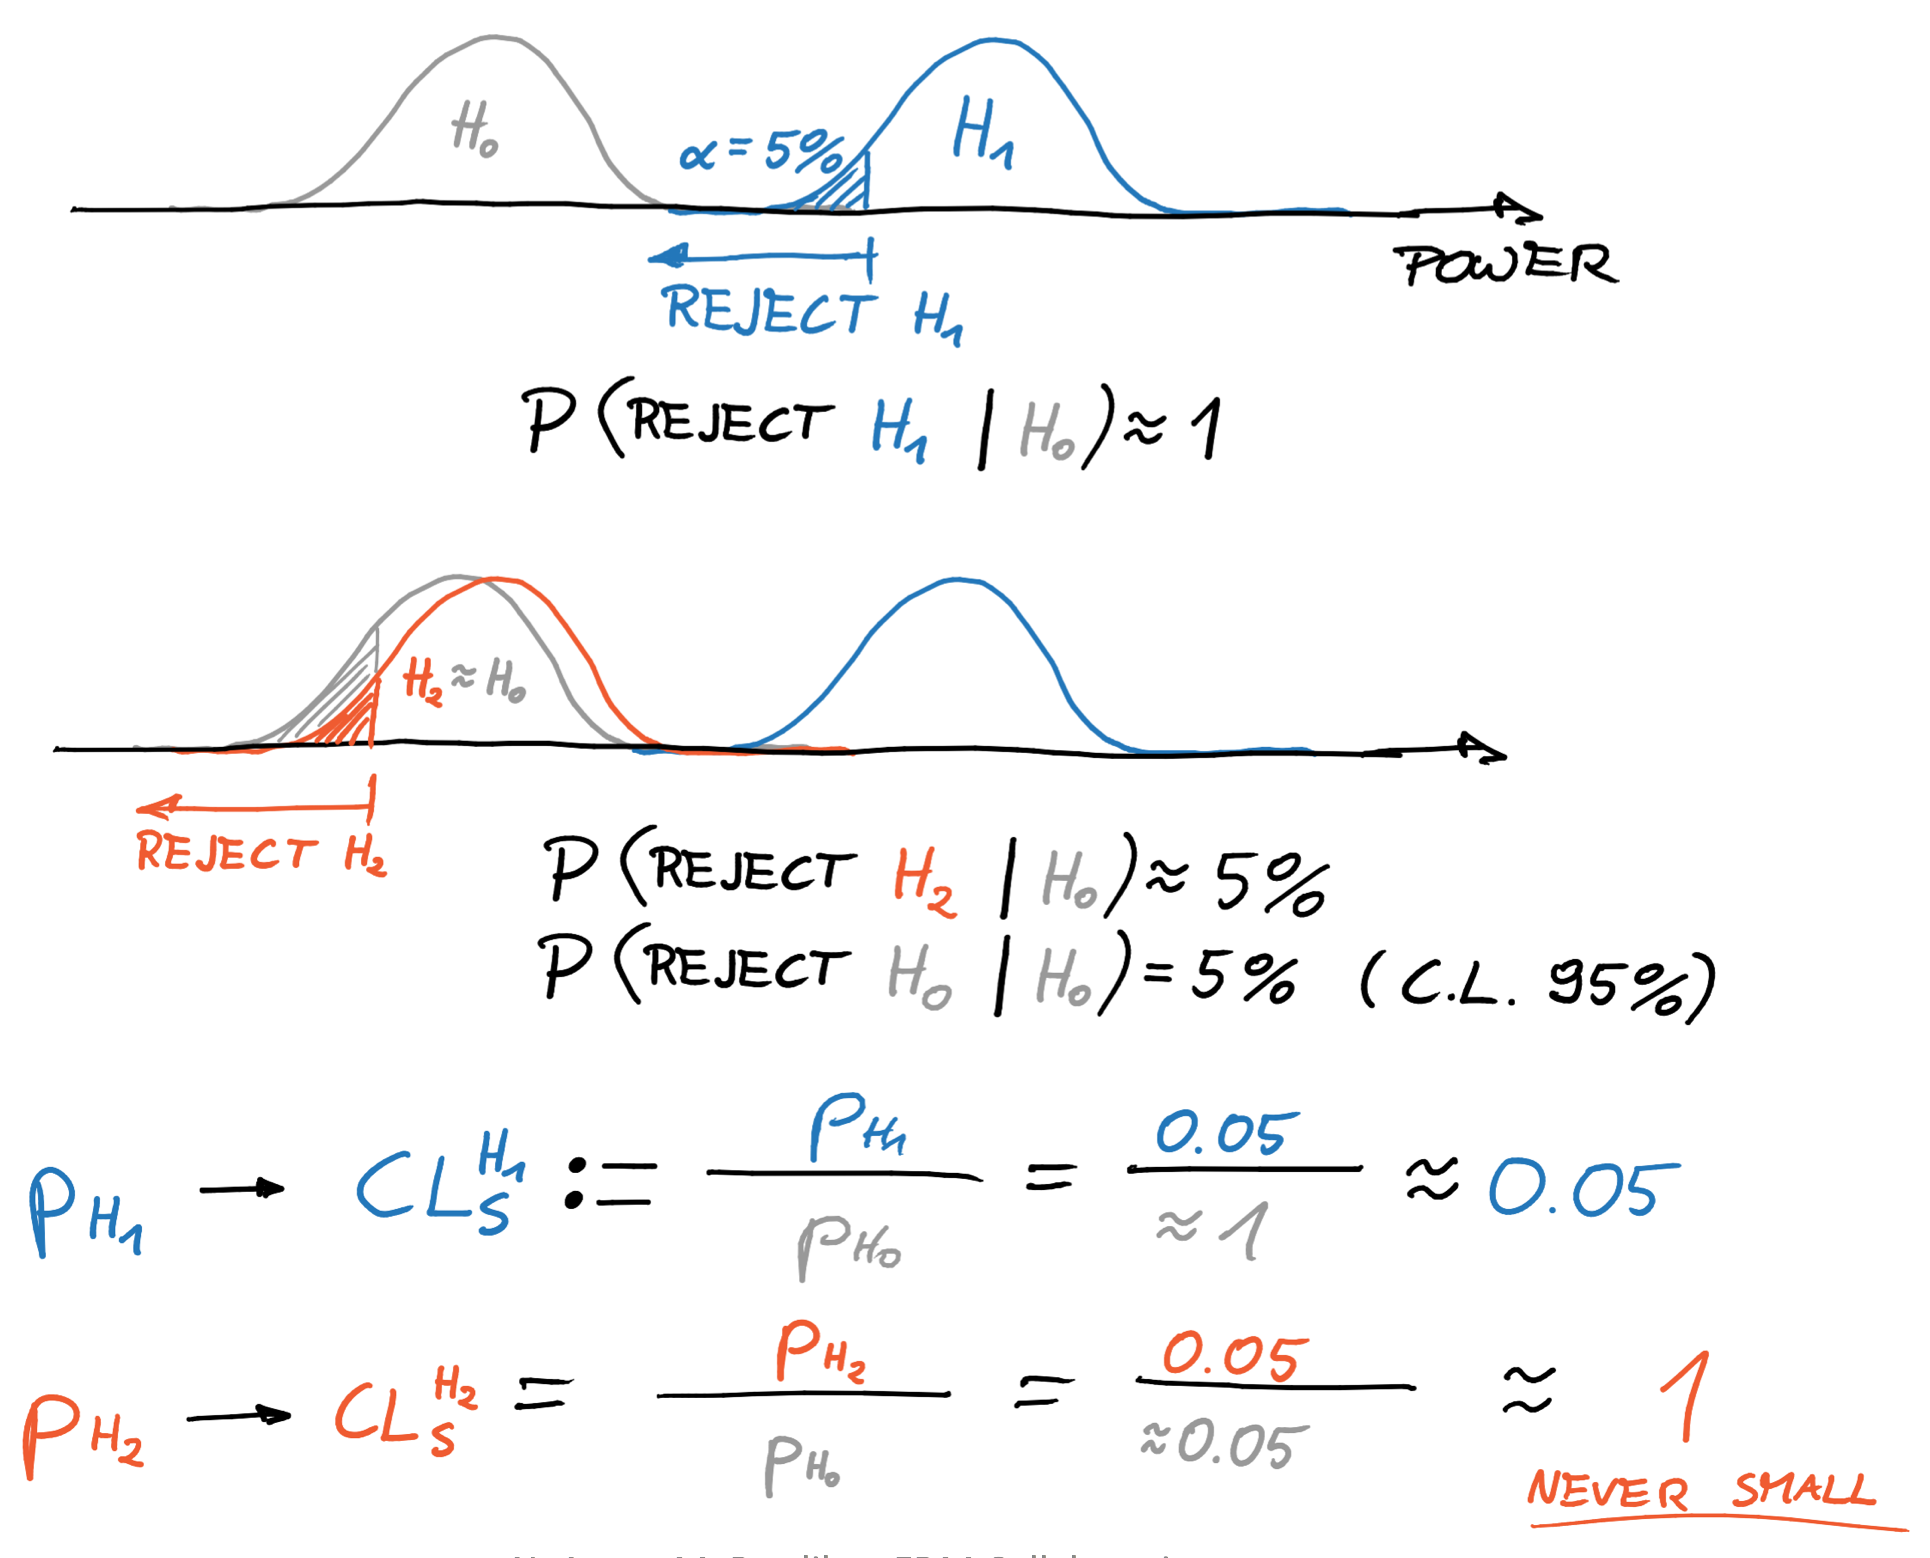
\includegraphics[width=0.8\linewidth]{gfx/axions/CLs.png}
  \caption{A graphical explanation of the motivation behind the CLs method. At the top: when the distributions of power for the null hypothesis $H_0$ and an alternative hypothesis $H_1$ are well separated, the probability of rejecting $H_1$ given $H_0$ is close to one. However, when we consider a signal of an arbitrarily small amplitude $H_2$, it still has roughly \SI{5}{\percent} chance to be rejected, on a \SI{95}{\percent} confidence level. If many of those are tested, \SI{5}{\percent} will be unjustifiably rejected. In the CLs method one considers, rather then the p-value of an alternative hypothesis, the ratio of it to the p-value of the null hypothesis. This imposes a statistical penalty to the hypotheses not well separated from the null one.}\label{fig:CLs}
\end{figure}

The black exclusion region in the left-hand side of Fig.\,\ref{fig:axions_exclusions} exhibits a number of thin peaks going down to very low amplitudes. Seemingly for some frequencies even tiny signals can be confidently excluded. This is disturbing, and rightfully so.
Consider, however, that as the power was evaluated for many frequencies, inevitably at some of them, roughly \SI{5}{\percent}, the power is low enough to be rejected at the \SI{95}{\percent} confidence level, even when tested against the distribution of power given the null hypothesis itself.
It is completely fine from the statistical point of view. Yet, a situation where a hypothesis is rejected based on a measurement which was not sensitive to it is uncomfortable.
One possible solution is called the \emph{CLs method}. The method is defined, as well as the problem itself is discussed in detail, in the booklet of the Particle Data Group~\cite{PDG2016}. Here, a short graphical explanation can be found in Fig.\,\ref{fig:CLs}. With use of the CLs method the exclusion is suppressed in the region of low sensitivity, as shown on the right-hand side i n Fig.\,\ref{fig:axions_exclusions}.

Rather than calculating each pixel of the alternative hypotheses space, one may resolve only the \SI{95}{\percent} C.L. threshold. This can be done, for example with the bisection algorithm run at each frequency.

The phase was treated as a nuisance parameter. In the MC simulations it was taken to be random, uniformly distributed between $0$ and $2\pi$. In general, though, the sensitivity may be phase-dependent. In particular, sensitivity for signals with periods much longer than the total span of the data set is linear for sin-like signals and quadratic for cos-like ones. This work does not consider the phase dependence and gives results with the phase marginalised.

In summary, there are three areas where the method looses sensitivity to detect oscillations, each with a different mechanism behind it. Most importantly, only signals with amplitude large enough to produce more power than noise can be excluded. Signals with periods longer than the total span of the data set are difficult to exclude, as only a small part of an oscillation is seen. Signals faster than the duration of a single measurement are integrated out, which reduces the sensitivity on the high-frequency side.




\section*{Periodograms -- Conclusion}
In this chapter the least squares spectral analysis, LSSA, was introduced as a method to look for oscillations in unevenly sampled time series with unequal error bars. The test of the null hypothesis (no signal present) gives an estimate of the level of confidence on which a discovery of an oscillating signal can be claimed. Then a space possible signals is explored to determine which ones can be excluded on the ground of not having been detected. In the next chapter this methodology is applied to the time series of the neutron electric dipole moment measurements performed at PSI\@. An oscillation there would be a hint of an axion dark matter.
